\documentclass[tikz,border=3.14mm]{standalone}
\usetikzlibrary{calc}
\begin{document}
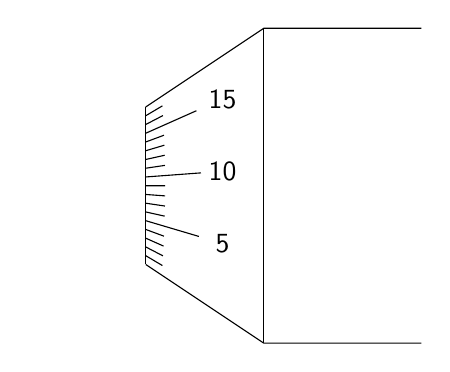
\begin{tikzpicture}[font=\sffamily]
 % \draw (0,0)--(-2,0) (0,-2)--(-2,-2);
 \draw[thin] (0,0)--(0,-2);
 \draw (0,0)coordinate (TL) --(1.5,1) coordinate (TR)  --(3.5,1) ;
 \draw (0,-2) coordinate (BL)--(1.5,-3)  coordinate (BR) --(3.5,-3) ;
 \draw[thin] (1.5,1)--(1.5,-3);
 % \draw (-2,-2) to[out=130,in=-130] (-2,-1) to[out=130,in=-130] (-2,0);
 % \draw[very thin] (-2,-1) to[out=50,in=-50] (-2,0);
 % \draw (3.5,1) to[out=-50,in=50] (3.5,-1) to[out=-50,in=50] (3.5,-3);
 % \draw[very thin] (3.5,-1) to[out=-130,in=130] (3.5,-3);
 \path (intersection cs:first line={(TL)--(TR)}, second line={(BL)--(BR)})
  coordinate (P);
 \clip (TL) -- (TR) -- (BR) -- (BL) -- cycle;
 \foreach \X [evaluate=\X as \Y using {int(mod(\X,5))}] in {1,...,17}
 {\ifnum\Y=0
   \draw[shorten >=-20pt] (P) -- (0,-2+\X/9) node[pos=1.65]{\X};
 \else
   \draw[shorten >=-7pt] (P) -- (0,-2+\X/9);
 \fi  }
\end{tikzpicture}
\end{document}
